As shown in Figure \ref{fig:map}, the mapping algorithm works well. This map was generated at Vanier College by manually driving the robot in an artificial environment. The environment was simply created by laying foldable tables and desk separators on the floor; thus, the obstacles used were big and could very easily be detected by the LiDAR sensor. While the mapping algorithm demonstrates promising results in a controlled environment, further testing in real-world settings is necessary.

Next, the Adaptive Monte Carlo Localization (AMCL) also works well. By providing the robot with an initial pose estimate within the pre-mapped environment, it can subsequently achieve precise and accurate localization after a brief period of motion. The repositioning of the robot in the map is very easily seen in RViz. Nevertheless, further testing with fully autonomous localization is needed.

Moreover, as of the time of writing this paper, there are still issues to be fixed with the global path planner. The robot is easily able to find and follow paths in large areas of free space; however, it cannot pass through narrower gaps. This is caused by the obstacles being too inflated. This can be simply fixed by changing the inflation parameter.

Lastly, the robot currently has issues with dead reckoning. As shown in Figure \ref{fig:dead-reckoning}, when moving towards a goal position with this navigation method, the robot stopped \qty{45}{cm} from the goal on the x-axis and \qty{35}{cm} from the goal on the y-axis. The percentage errors can be calculated as follows:
\begin{equation*}
    \begin{split}
        \% error_x & =\left|\frac{d_\text{actual}-d_\text{experimental}}{d_\text{actual}}\right|\times100\% \\
                   & =\left|\frac{\qty{3}{m}-(\qty{3}{m}-\qty{0.45}{m})}{\qty{3}{m}}\right|\times100\%      \\
                   & =15\%
    \end{split}
\end{equation*}
\begin{equation*}
    \begin{split}
        \% error_y & =\left|\frac{d_\text{actual}-d_\text{experimental}}{d_\text{actual}}\right|\times100\% \\
                   & =\left|\frac{\qty{0}{m}-\qty{0.35}{m}}{\qty{0}{m}}\right|\times100\%                   \\
                   & = \text{DNE}
    \end{split}
\end{equation*}
These significant errors are caused by two factors. First, there is wheel slippage due to the very smooth floor. Thus, a rougher floor may improve the results. Second, the dead reckoning algorithm produces very low wheel velocities at the beginning and end of the trajectory. Since these velocities are rounded to 0, the robot does not move and error is introduced. A solution addressing this problem has yet to be found.

\begin{figure}[!htb]
    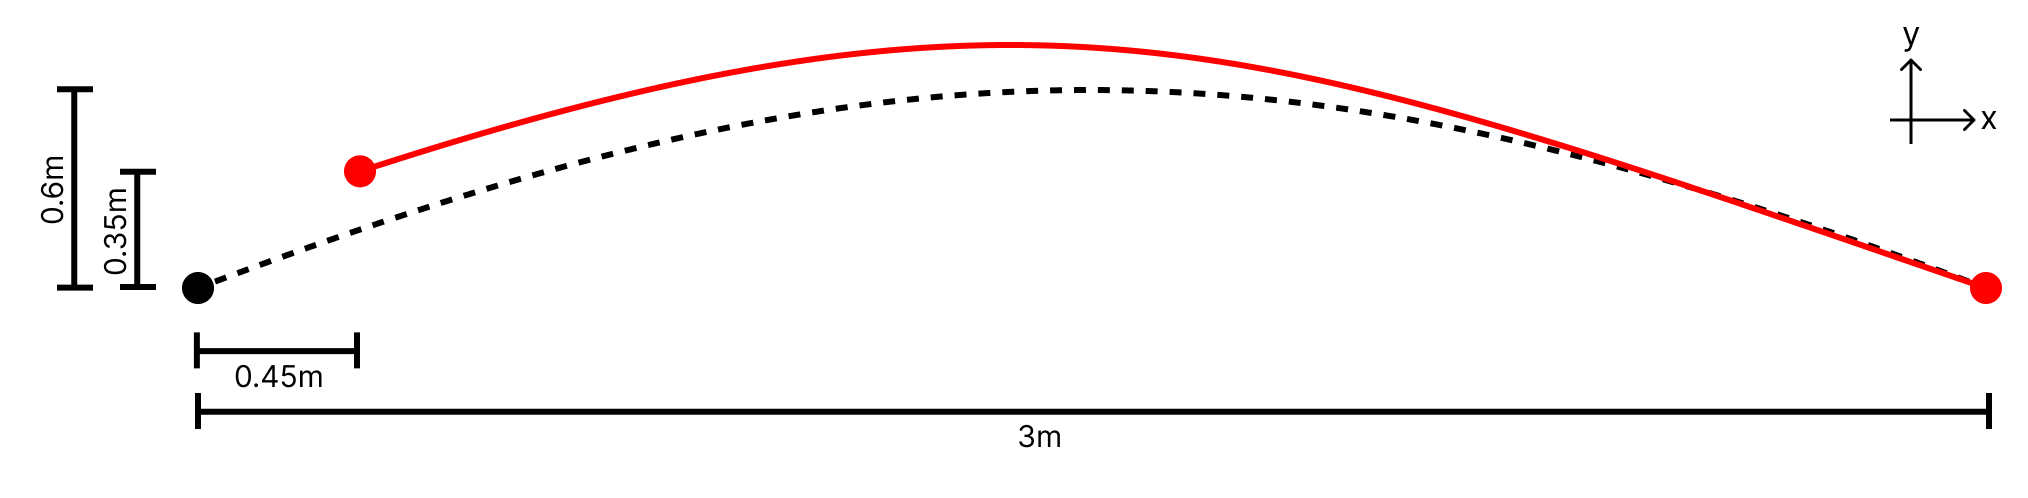
\includegraphics[width=12cm]{dead-reckoning.jpg}
    \centering
    \caption{Representation of the dead-reckoning test. The black dotted path is the intended path, while the red continuous path is the actual path of the robot.}
    \label{fig:dead-reckoning}
\end{figure}